In this chapter, we present the results following the methodology described in Chapter~\ref{chapter:methodology}. We first present the results of the data exploration, preprocessing and augmentation. We then present the results of the automated evaluation, including topic coherence scores, topic diversity scores, silhouette scores, comparison with baseline models, and hyperparameter tuning. Then, we show the tag generation pipeline, including the base BERTopic model and its subcomponents and hyperparameters, the additional fine-tuning model, and zeroshot classifier. Finally, we present the results of the human evaluation, followed by the results of the large-scale automated evaluation.

\section{Data exploration, preprocessing and augmentation}
Following an initial exploratory data analysis, we identified several methods for augmenting the dataset descriptions. The dataset descriptions are augmented with the following additional information:

\begin{itemize}
\item \textbf{Tags} — The generated tags that have already been created for the dataset.
\item \textbf{Name} — The name of the dataset.
\item \textbf{Features} — The names of the dataset's features (columns).
\item \textbf{Scraped text} — For some datasets, we scrape text from the original sources and append it to the dataset description.
\end{itemize}

Additionally, we remove all datasets that have a cosine similarity of 0.99 or higher with another dataset, as these datasets are likely to be duplicates or different versions of the same dataset. This results in the removal of ~300 datasets from the original 5500 datasets.

After augmenting the dataset descriptions, we observe that the augmented descriptions are longer, and potentially more informative, as illustrated in \cref{fig:description_vs_augmented_description.png}. All subsequent analyses are performed on the augmented dataset descriptions.

\begin{figure}[h]
    \centering
    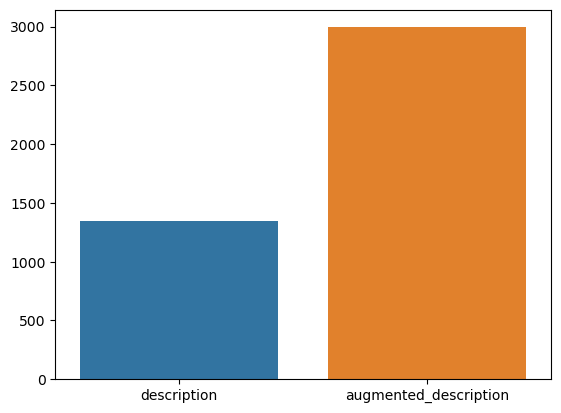
\includegraphics[width=0.5\textwidth]{figures/description_vs_augmented_description.png}
    \caption{Histogram of the length of dataset descriptions vs augmented dataset descriptions}
    \label{fig:description_vs_augmented_description.png}
\end{figure}

Additionally, we find that OpenML datasets can have multiple versions. Our analysis of dataset versions reveals that most datasets have only 2 versions, though several datasets have more than 2 (\cref{fig:number_of_versions}).
\begin{figure}[h]
    \centering
    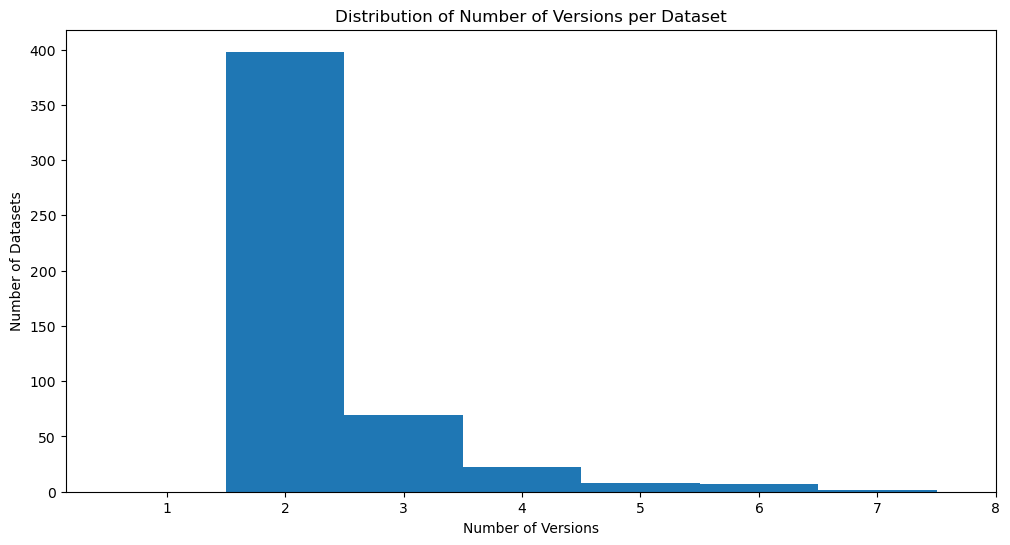
\includegraphics[width=0.5\textwidth]{figures/number_of_versions.png}
    \caption{Histogram of the number of versions of dataset descriptions}
    \label{fig:number_of_versions}
\end{figure}

We also examine the similarity between different versions of the datasets. Our analysis shows that most datasets have a cosine similarity of 0.9 or higher, suggesting that the versions are highly similar to one another (\cref{fig:cosine_similarity_dataset_versions}).

\begin{figure}[h]
    \centering
    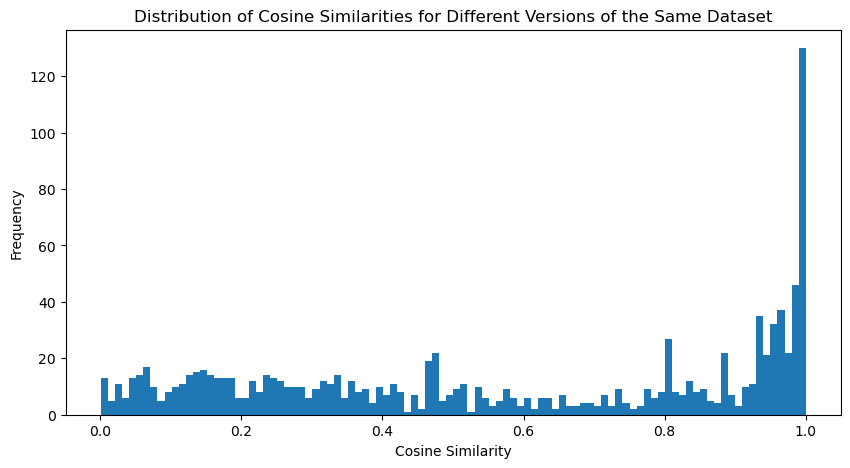
\includegraphics[width=0.5\textwidth]{figures/cosine_similarity_dataset_versions.png}
    \caption{Histogram of the cosine similarity of different versions of dataset descriptions}
    \label{fig:cosine_similarity_dataset_versions}
\end{figure}

In the exploratory data analysis subsection, we present the most relevant statistics about the OpenML datasets. All further findings are based on the augmented descriptions, rather than the original ones. For readers seeking more detailed statistics, additional information can be found in the \href{https://github.com/ivangermanov/openml-tags}{GitHub repository} \cite{germanov_topic_modeling_of_2024}.

\cref{fig:length_of_descriptions} presents a histogram depicting the length of dataset descriptions. The lengths range from 0 to 10,000 words, with the majority of descriptions being under 5,000 words. A few outliers exceed 10,000 words.

\begin{figure}[h]
    \centering
    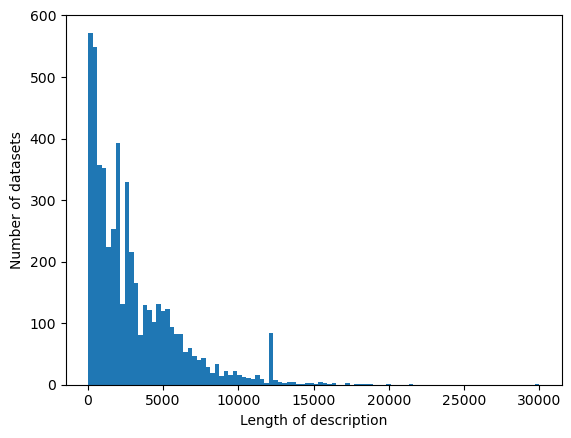
\includegraphics[width=0.5\textwidth]{figures/length_of_descriptions.png}
    \caption{Histogram of the length of dataset descriptions}
    \label{fig:length_of_descriptions}
\end{figure}

Similarly, \cref{fig:words_of_descriptions} and \cref{fig:sentences_of_descriptions} display comparable distributions, this time for the number of words and the number of sentences, respectively.

\begin{figure}[h]
    \centering
    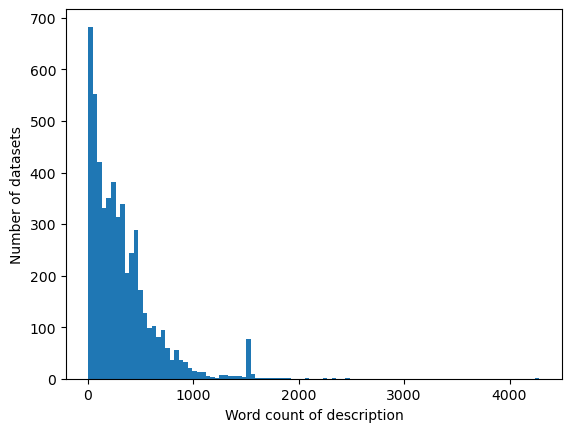
\includegraphics[width=0.5\textwidth]{figures/words_of_descriptions.png}
    \caption{Histogram of the number of words of dataset descriptions}
    \label{fig:words_of_descriptions}
\end{figure}

\begin{figure}[h]
    \centering
    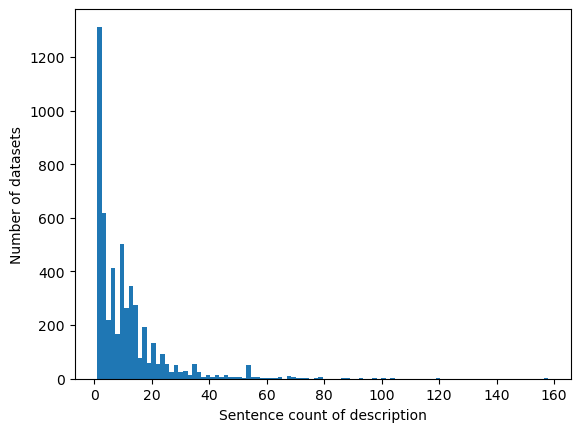
\includegraphics[width=0.5\textwidth]{figures/sentences_of_descriptions.png}
    \caption{Histogram of the number of sentences of dataset descriptions}
    \label{fig:sentences_of_descriptions}
\end{figure}

From these histograms, we can infer that the dataset descriptions are relatively short, with the majority being comparable in length to two Twitter tweets. This is important to note, as descriptions that are too short may lack enough information to generate meaningful tags. However, this may not necessarily pose an issue, as prior studies have successfully applied topic modeling to tweets and other short texts \cite{cataldi_emerging_2010, churchill_percolation-based_2020, curiskis_evaluation_2020, kasiviswanathan_emerging_2011, paul_discovering_2014, yin_dirichlet_2014}.

We applied Named Entity Recognition (NER) and Part-of-Speech (POS) tagging to the dataset descriptions to identify the most common entities and parts of speech (\cref{fig:pos,fig:ner}). A significant number of words were tagged as \textit{X}, indicating that the POS tagger was unable to determine the part of speech for these words. This is likely due to the presence of domain-specific terms not included in the POS tagger's vocabulary, as well as unrecognized or anomalous tokens and symbols. Additionally, we found that the most frequent named entity is \textit{PERSON}, which can be attributed to the fact that many dataset descriptions reference the names of dataset authors or associated papers. Both of these findings pose challenges for the performance of the tag generation model, as unrecognized tokens and author names do not contribute meaningful information for generating relevant tags.

\begin{figure}[h]
    \centering
    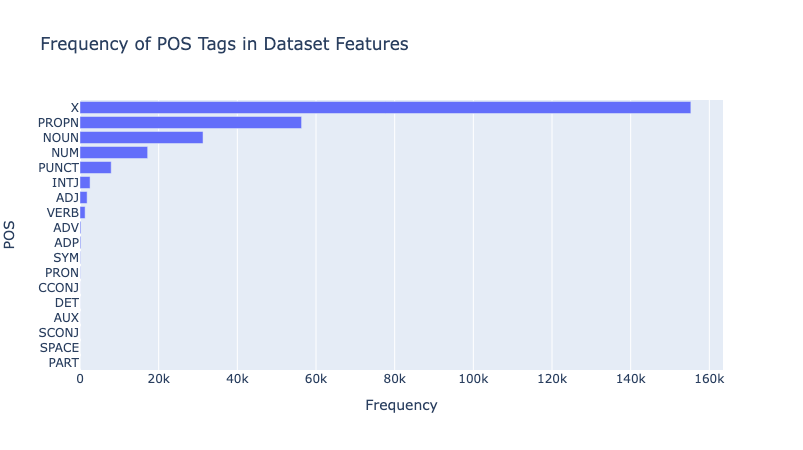
\includegraphics[width=0.55\textwidth]{figures/pos.png}
    \caption{Bar chart of the most common parts of speech in dataset descriptions}
    \label{fig:pos}
\end{figure}

\begin{figure}[h]
    \centering
    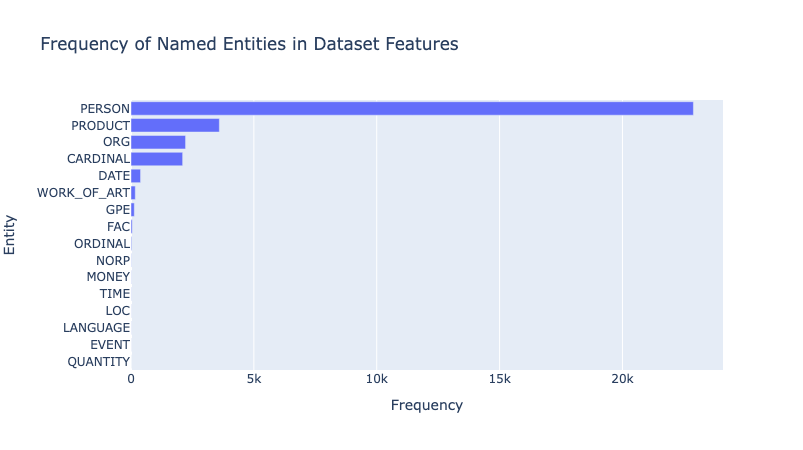
\includegraphics[width=0.55\textwidth]{figures/ner.png}
    \caption{Bar chart of the most common named entities in dataset descriptions}
    \label{fig:ner}
\end{figure}

We also examine how many datasets include URLs to original sources in their descriptions (\cref{fig:original_data_url_vs_no}). A significant number of datasets contain URLs, which could be used to scrape additional text for augmenting the descriptions. However, upon closer inspection, we find that the information in these URLs is often redundant with what is already provided in the dataset descriptions. Nonetheless, for some datasets, the URLs contain supplementary information that could be valuable for generating tags, which we then scrape.

\begin{figure}[h]
    \centering
    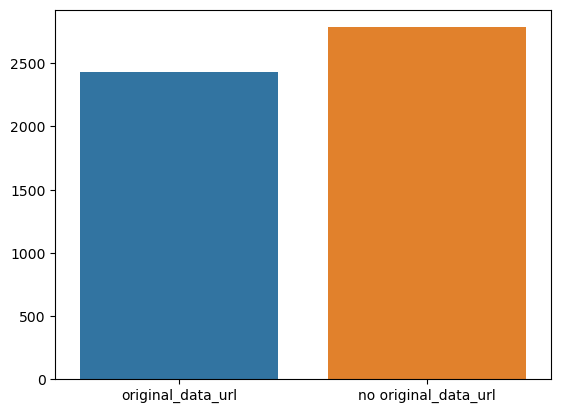
\includegraphics[width=0.5\textwidth]{figures/original_data_url_vs_no.png}
    \caption{Bar chart of the number of datasets with and without URLs to original sources}
    \label{fig:original_data_url_vs_no}
\end{figure}

\section{Automated Evaluation Results}
\subsection{Topic coherence scores}

\subsection{Topic diversity scores}

\subsection{Silhouette scores}

\subsection{Comparison with baseline models}

\subsection{Hyperparameter tuning}

\section{Tag Generation Pipeline}
\subsection{Base BERTopic Model}
\subsection{Fine-tuning Results}
\subsection{Zeroshot Classifier Performance}


\section{Human Evaluation Results}
\subsection{Relevance Ratings}
\subsection{Generality Ratings}
\subsection{Coverage Ratings}
\subsection{Shared Coverage Ratings}
\subsection{Intruder Detection Task Results}
\subsection{Inter-rater Reliability Analysis}

\section{Large-scale Automated Evaluation Results}
\subsection{GPT-4-mini Intruder Detection Results}
\subsection{GPT-4-mini Tag Quality Assessment Results}
\subsection{Comparison with Human Evaluation Results}

\section{Model Robustness and Generalizability}
\subsection{Performance Across Different Document Types}
\subsection{Consistency of Tag Generation}

\section{Summary of Key Findings}